% =====================================================================
% Supplementary material for "SceneMiner: What Survives an Audit of
% Language-Guided Hard-Scene Mining for Autonomous Driving".
% Tables under supp_tables/ are generated by scripts/make_supp_tables.py;
% figures by scripts/make_figures.py. Nothing here is typed by hand from
% memory except the hyperparameter table, which mirrors the code defaults.
% =====================================================================
\documentclass[10pt,letterpaper]{article}
\usepackage[margin=0.8in]{geometry}
\usepackage{times,graphicx,amsmath,amssymb,booktabs,longtable,array}
\usepackage{caption}
\usepackage[colorlinks,linkcolor=black,citecolor=black,urlcolor=black]{hyperref}
\captionsetup{font=small,labelfont=bf}
\renewcommand{\thetable}{S\arabic{table}}
\renewcommand{\thefigure}{S\arabic{figure}}
\renewcommand{\thesection}{S\arabic{section}}
\setlength{\LTcapwidth}{\textwidth}

\title{SceneMiner: What Survives an Audit of Language-Guided Hard-Scene Mining\\
       \large Supplementary Material}
\author{}
\date{}

\begin{document}
\maketitle

\noindent This supplement gives the full specification of SceneMiner v2.3, the
human annotation protocols, the complete significance table for the CAM\_FRONT
study, per-query results for every evaluated query, the list of training queries,
and additional qualitative retrievals.

% =====================================================================
\section{Architecture and hyperparameters}
% =====================================================================

\begin{table}[h]\centering\small
\caption{\textbf{SceneMiner v2.3 specification.} Values are the code defaults
used for every reported run (\texttt{src/scene\_mining/filter/sceneminer\_v2\_3.py},
\texttt{scripts/train\_sceneminer\_v23.py}).}
\label{tab:hp}
\begin{tabular}{lll}
\toprule
group & parameter & value\\
\midrule
Stage-1 inputs & BEV embedding $\mathbf{e}$ / tags $\mathbf{t}$ / risk $r$ & $256$ / $20$ / $1$\\
 & Qwen visual token $\mathbf{v}$ / SigLIP2 image / margins $\mathbf{m}$ & $2048$ / $768$ / $4$\\
 & metadata prior $\pi$ & $26$ ($20$ tag $z$-scores $+$ $6$ one-hots)\\
Fusion & $d_{\mathrm{model}}$, heads, decoder layers & $256$, $4$, $2$ (pre-norm)\\
 & FiLM query conditioning, type embeddings & yes, $6$ token types\\
 & bilinear rank, dropout, score temperature & $64$, $0.1$, $0.30$\\
Base & \textsc{PartNorm} momentum, $\epsilon$ & $0.01$, $10^{-5}$\\
 & router temperature, entropy cap & $1.0$, $\max_k w_k\le0.70$\\
Concept gate & $T_a$ (column alignment) & $0.10$\\
 & $\tau_c$, $T_c$ (from label-free banks) & $0.245$, $0.046$\\
 & in-vocabulary / OOV bank & $72$ training phrasings / $12$ generic phrases\\
Residual & \textsc{ResNorm} bound $\alpha$ & $0.5$\\
FN rescue & cosine threshold, margin floor & $+1.0\sigma$, $-0.5\sigma$\\
Optimisation & optimiser, learning rate, weight decay & AdamW, $10^{-4}$, $0.01$\\
 & schedule & linear warm-up $200$ steps, cosine to $10^{-7}$\\
 & steps, gradient clip & $3000$, $1.0$\\
 & batch & $4$ queries $\times$ ($2$ pos.\ $+$ $2$ cond.\ neg.)\\
Loss & listwise InfoNCE, margin-confidence weights & $\tanh(|m|)$\\
 & conditional hinge weight, margin & $4.0$, $1.0$\\
 & entropy-floor weight $\lambda_{\mathrm{ent}}$ & $2.0$\\
Anti-shortcut & margin dropout / 3D dropout (per step) & $50\%$ / $30\%$\\
 & agreement-distillation floor & $0.30$\\
Model & trainable parameters & $4{,}678{,}736$\\
 & seeds & $5$ (scores averaged)\\
 & latency, $1508$ scenes, one query, A40 & $6.77\pm0.32$\,ms\\
\bottomrule
\end{tabular}
\end{table}

\paragraph{Canonical concept descriptions.} ``water droplets on camera lens'',
``bright headlight or sun glare'', ``wet reflective road surface'', ``dark low
contrast poor visibility''.

\paragraph{Out-of-vocabulary bank.} ``a parking lot'', ``a roundabout'', ``a
tunnel entrance'', ``a bridge over a river'', ``a gas station'', ``a suburban
cul-de-sac'', ``a toll booth'', ``a railway crossing'', ``a school zone sign'',
``a freeway on-ramp'', ``a shopping mall entrance'', ``a narrow alley between
buildings''. It was fixed before any evaluation query was written and contains
no weather words and none of the Stratum-5 categories.

\paragraph{Label-free scale evidence.} During training the running standard
deviations of the three base parts converge to $0.031$ (cosine), $0.566$
(margin) and $0.159$ (prior), and that of the raw residual to $6.31$. Both incommensurabilities
of the main paper are therefore visible without any label.

% =====================================================================
\section{Why the 150-query suite is circular}
\label{sec:supp-circ}
% =====================================================================

Relevance in the 390-query suite is a conjunction over cached attributes:
lighting and weather from the nuScenes/Waymo metadata, density from 3D boxes, and
the four degradation flags from the Stage-1 VLM. An index reading the same
attributes therefore scores $1.000$~mAP. Per-query results on this suite
(Table~\ref{tab:pq-suite}) measure agreement with the VLM, and gains there
partly reflect sharper alignment with the correct VLM column. Human-graded
evidence is in the main paper's Tables~1, 3, 7 and~8.

% =====================================================================
\section{Human annotation protocols}
% =====================================================================

\paragraph{Degradation labels (rater 1, 600 scenes).} A zero-dependency
browser tool (\texttt{scripts/annotate\_ui.py}, Python standard library only)
shows one CAM\_FRONT keyframe at a time from a frozen random sample of the
evaluation split, stratified so that VLM-positive, VLM-negative and
near-threshold scenes are all represented. The rater toggles four attributes
with keys \texttt{1}--\texttt{4} and saves with \texttt{Enter}; \texttt{b} goes
back, \texttt{u} marks a scene unsure, \texttt{s} skips it. Every scene is
autosaved. VLM outputs are never shown. Of $600$ scenes, $550$ remain after
removing unsure scenes and skipped scenes with ambiguous labels (``Mode B'').
Figure~\ref{fig:ui} shows the interface on a real labelled scene.

\begin{figure}[h]\centering
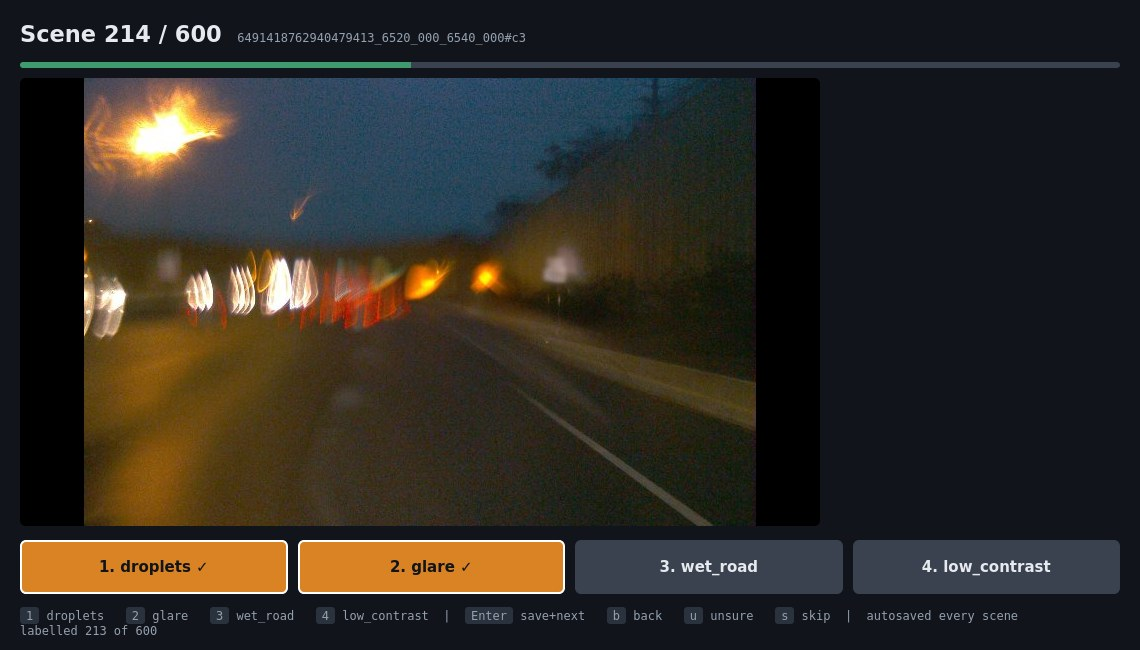
\includegraphics[width=0.8\textwidth]{figures/supp_annotation_ui.jpg}
\caption{\textbf{The annotation interface}, rendered with one real scene and the
labels the rater recorded for it (droplets and glare). The page markup and
script are the tool's own; for this capture the scene record was inlined instead
of fetched, because the headless browser captures before an asynchronous fetch
completes.}
\label{fig:ui}
\end{figure}

\paragraph{Stratum-5 semantic labels.} Extracted by
\texttt{scripts/extract\_human\_semantic\_gt.py} from the official nuScenes
tables only. An object counts if it lies inside the CAM\_FRONT field of view
($|\text{azimuth}|\le32.6^\circ$ in the ego frame, from the camera intrinsics)
with visibility level $\ge2$ ($>40\%$). A scene flag is set if the condition holds
in $\ge25\%$ of the scene's annotated keyframes; per-scene fractions are released
so other thresholds can be checked.

\begin{table}[h]\centering\small
\caption{\textbf{Stratum-5 flag definitions} and prevalence among the $700$
corpus and $150$ val scenes.}
\label{tab:flags}
\begin{tabular}{p{2.6cm}p{9.0cm}rr}
\toprule
flag & definition (front sector, visibility $>40\%$) & corpus & val150\\
\midrule
pedestrian\_close & adult, child, construction-worker or police pedestrian within $25$\,m & $230$ & $35$\\
vru & bicycle or motorcycle with the \texttt{cycle.with\_rider} attribute within $40$\,m, or any pedestrian within $15$\,m & $119$ & $26$\\
construction\_zone & $\ge3$ traffic cones, or a cone together with a barrier, or a construction worker or construction vehicle, within $40$\,m. Barriers alone do not count: they line ordinary roads throughout nuScenes & $142$ & $26$\\
heavy\_vehicle & rigid or bendy bus, truck, trailer or construction vehicle within $25$\,m & $149$ & $36$\\
rare\_or\_child & child, stroller, wheelchair, police officer, emergency vehicle, debris or pushable/pullable object within $40$\,m & $84$ & $22$\\
night / rain & word in the human-written scene description & $84$ / $138$ & $15$ / $27$\\
\bottomrule
\end{tabular}
\end{table}

% =====================================================================
\section{All 30 front-sector significance tests}
% =====================================================================

\begin{longtable}{l r l r r r r l r l}
\caption{All 30 CAM\_FRONT-sector tests (Milestone 11), sorted by $p$. 150 uncontaminated val scenes; bootstrap CI over scenes (1000); permutation $p$ (1000); Benjamini--Hochberg $q$ over the full family. $^{**}q<0.05$, $^{*}q<0.10$.}\label{tab:bh}\\
\toprule
partition & $n_{deg}$ & metric & degraded & clean & $\Delta$ & $\sigma$ & 95\,\% CI & $p$ & $q$\\
\midrule
\endfirsthead
\toprule
partition & $n_{deg}$ & metric & degraded & clean & $\Delta$ & $\sigma$ & 95\,\% CI & $p$ & $q$\\
\midrule
\endhead
\bottomrule
\endfoot
any\_degradation & 42 & mAP\_front & 0.3886 & 0.4792 & -0.0906 & -0.69 & [-0.140, -0.038] & 0.001 & 0.015$^{**}$\\
droplets & 34 & mAP\_front & 0.3791 & 0.4773 & -0.0982 & -0.74 & [-0.152, -0.039] & 0.001 & 0.015$^{**}$\\
wet\_road & 34 & mAP\_front & 0.3910 & 0.4730 & -0.0820 & -0.62 & [-0.138, -0.019] & 0.006 & 0.045$^{**}$\\
any\_degradation & 42 & fp\_rate & 0.3503 & 0.2775 & +0.0729 & +0.50 & [+0.012, +0.142] & 0.006 & 0.045$^{**}$\\
any\_degradation & 42 & recall\_near & 0.7703 & 0.8262 & -0.0559 & -0.44 & [-0.108, -0.004] & 0.019 & 0.080$^{*}$\\
droplets & 34 & recall\_near & 0.7650 & 0.8248 & -0.0598 & -0.47 & [-0.119, -0.001] & 0.020 & 0.080$^{*}$\\
any\_degradation & 42 & mATE\_front & 0.8330 & 0.7553 & +0.0777 & +0.44 & [+0.004, +0.150] & 0.022 & 0.080$^{*}$\\
wet\_road & 34 & fp\_rate & 0.3469 & 0.2835 & +0.0634 & +0.43 & [+0.001, +0.131] & 0.022 & 0.080$^{*}$\\
any\_degradation & 42 & recall\_far & 0.5312 & 0.6079 & -0.0767 & -0.42 & [-0.142, -0.006] & 0.024 & 0.080$^{*}$\\
low\_contrast & 24 & fp\_rate & 0.3529 & 0.2874 & +0.0655 & +0.45 & [-0.024, +0.166] & 0.030 & 0.087$^{*}$\\
low\_contrast & 24 & recall\_far & 0.5042 & 0.6014 & -0.0973 & -0.53 & [-0.184, -0.008] & 0.032 & 0.087$^{*}$\\
droplets & 34 & mATE\_front & 0.8320 & 0.7596 & +0.0724 & +0.41 & [-0.004, +0.149] & 0.035 & 0.087$^{*}$\\
droplets & 34 & recall\_far & 0.5361 & 0.6030 & -0.0669 & -0.37 & [-0.144, +0.006] & 0.056 & 0.129\\
wet\_road & 34 & recall\_near & 0.7759 & 0.8212 & -0.0453 & -0.35 & [-0.105, +0.012] & 0.089 & 0.178\\
wet\_road & 34 & mATE\_front & 0.8233 & 0.7628 & +0.0605 & +0.34 & [-0.022, +0.140] & 0.089 & 0.178\\
low\_contrast & 24 & mAP\_front & 0.4123 & 0.4621 & -0.0499 & -0.38 & [-0.119, +0.025] & 0.101 & 0.189\\
wet\_road & 34 & recall\_far & 0.5421 & 0.6007 & -0.0585 & -0.32 & [-0.127, +0.013] & 0.107 & 0.189\\
droplets & 34 & mAOE\_front & 0.5219 & 0.4282 & +0.0937 & +0.29 & [-0.052, +0.260] & 0.143 & 0.238\\
glare & 6 & mAP\_front & 0.3803 & 0.4579 & -0.0776 & -0.59 & [-0.162, +0.021] & 0.162 & 0.256\\
glare & 6 & mAOE\_front & 0.6167 & 0.4426 & +0.1740 & +0.54 & [-0.138, +0.588] & 0.183 & 0.265\\
droplets & 34 & fp\_rate & 0.3274 & 0.2892 & +0.0382 & +0.26 & [-0.017, +0.091] & 0.186 & 0.265\\
any\_degradation & 42 & mAOE\_front & 0.5008 & 0.4308 & +0.0701 & +0.22 & [-0.067, +0.203] & 0.233 & 0.317\\
wet\_road & 34 & mAOE\_front & 0.4914 & 0.4377 & +0.0536 & +0.17 & [-0.098, +0.212] & 0.402 & 0.524\\
glare & 6 & recall\_far & 0.5362 & 0.5896 & -0.0534 & -0.29 & [-0.195, +0.068] & 0.480 & 0.599\\
low\_contrast & 24 & recall\_near & 0.7961 & 0.8137 & -0.0176 & -0.14 & [-0.084, +0.045] & 0.566 & 0.680\\
low\_contrast & 24 & mATE\_front & 0.7943 & 0.7731 & +0.0212 & +0.12 & [-0.083, +0.120] & 0.612 & 0.706\\
low\_contrast & 24 & mAOE\_front & 0.4203 & 0.4548 & -0.0345 & -0.11 & [-0.199, +0.143] & 0.635 & 0.706\\
glare & 6 & mATE\_front & 0.7533 & 0.7772 & -0.0240 & -0.14 & [-0.106, +0.060] & 0.733 & 0.786\\
glare & 6 & fp\_rate & 0.3147 & 0.2972 & +0.0175 & +0.12 & [-0.035, +0.090] & 0.762 & 0.789\\
glare & 6 & recall\_near & 0.8228 & 0.8106 & +0.0122 & +0.10 & [-0.071, +0.089] & 0.816 & 0.816\\
\end{longtable}


% =====================================================================
\section{Per-query results}
% =====================================================================

The 390-query suite has $240$ training and $150$ evaluation queries; Stratum~5
adds $40$, for $430$ in total. The $190$ evaluated queries are scored below. The
$240$ training queries are listed in \S\ref{sec:train} but never scored, because
SceneMiner's head saw their text during training.

{\footnotesize
\begin{longtable}{r l p{5.0cm} p{3.4cm} r r r r}
\caption{Per-query mAP, 150 evaluation queries of the 390-query suite, 602 eval-split scenes. Relevance is a predicate over cached VLM attributes (circular; \S\ref{sec:supp-circ}). Lookup reads the column of the attribute the predicate names; -- where it names none.}\label{tab:pq-suite}\\
\toprule
\# & S & query & predicate & pos & SceneMiner & SigLIP2 & lookup\\
\midrule
\endfirsthead
\toprule
\# & S & query & predicate & pos & SceneMiner & SigLIP2 & lookup\\
\midrule
\endhead
\bottomrule
\endfoot
1 & S1 & a few water specks on the lens & droplets=T & 119 & 0.966 & 0.788 & 1.000\\
2 & S1 & light droplets scattered on the lens & droplets=T & 119 & 0.964 & 0.795 & 1.000\\
3 & S1 & water droplets smearing the camera lens & droplets=T & 119 & 0.958 & 0.888 & 1.000\\
4 & S1 & rain beading across the lens & droplets=T & 119 & 0.964 & 0.886 & 1.000\\
5 & S1 & a faint halo around a street light & glare=T & 40 & 0.907 & 0.216 & 1.000\\
6 & S1 & mild light flare at the frame edge & glare=T & 40 & 0.905 & 0.480 & 1.000\\
7 & S1 & noticeable glare washing across the image & glare=T & 40 & 0.930 & 0.381 & 1.000\\
8 & S1 & specular glare washing out the image & glare=T & 40 & 0.935 & 0.527 & 1.000\\
9 & S1 & a lightly damp road surface & wet\_road=T & 124 & 0.991 & 0.560 & 1.000\\
10 & S1 & patchy wet tarmac & wet\_road=T & 124 & 0.990 & 0.615 & 1.000\\
11 & S1 & wet reflective asphalt after rainfall & wet\_road=T & 124 & 0.989 & 0.810 & 1.000\\
12 & S1 & slick wet pavement throwing reflections & wet\_road=T & 124 & 0.990 & 0.747 & 1.000\\
13 & S1 & slightly flat lighting & low\_contrast=T & 103 & 0.856 & 0.388 & 1.000\\
14 & S1 & a dim view where shapes lose definition & low\_contrast=T & 103 & 0.971 & 0.160 & 1.000\\
15 & S1 & hazy washed out view with unclear boundaries & low\_contrast=T & 103 & 0.966 & 0.372 & 1.000\\
16 & S1 & poor visibility with objects blending in & low\_contrast=T & 103 & 0.969 & 0.399 & 1.000\\
17 & S1 & a few water specks on the lens at night & droplets=T, lighting=night & 31 & 0.785 & 0.655 & 0.283\\
18 & S1 & a few water specks on the lens in daylight & droplets=T, lighting=day & 78 & 0.886 & 0.653 & 0.675\\
19 & S1 & a few water specks on the lens in rain & droplets=T, weather=rain & 55 & 0.988 & 0.664 & 0.566\\
20 & S1 & a few water specks on the lens in dense traffic & droplets=T, density=dense & 82 & 0.795 & 0.511 & 0.739\\
21 & S1 & a few water specks on the lens on an empty road & droplets=T, density=sparse & 10 & 0.056 & 0.059 & 0.066\\
22 & S1 & light droplets scattered on the lens at night & droplets=T, lighting=night & 31 & 0.790 & 0.757 & 0.283\\
23 & S1 & light droplets scattered on the lens in daylight & droplets=T, lighting=day & 78 & 0.712 & 0.455 & 0.675\\
24 & S1 & light droplets scattered on the lens in rain & droplets=T, weather=rain & 55 & 0.857 & 0.511 & 0.566\\
25 & S1 & light droplets scattered on the lens in dense traffic & droplets=T, density=dense & 82 & 0.665 & 0.413 & 0.739\\
26 & S1 & light droplets scattered on the lens on an empty road & droplets=T, density=sparse & 10 & 0.226 & 0.170 & 0.066\\
27 & S1 & water droplets smearing the camera lens at night & droplets=T, lighting=night & 31 & 0.750 & 0.724 & 0.283\\
28 & S1 & water droplets smearing the camera lens in daylight & droplets=T, lighting=day & 78 & 0.892 & 0.788 & 0.675\\
29 & S1 & water droplets smearing the camera lens in rain & droplets=T, weather=rain & 55 & 0.994 & 0.687 & 0.566\\
30 & S1 & water droplets smearing the camera lens in dense traffic & droplets=T, density=dense & 82 & 0.799 & 0.697 & 0.739\\
31 & S1 & water droplets smearing the camera lens on an empty road & droplets=T, density=sparse & 10 & 0.052 & 0.052 & 0.066\\
32 & S1 & a faint halo around a street light at night & glare=T, lighting=night & 9 & 0.870 & 0.119 & 0.263\\
33 & S1 & a faint halo around a street light in daylight & glare=T, lighting=day & 25 & 0.596 & 0.223 & 0.628\\
34 & S1 & a faint halo around a street light in rain & glare=T, weather=rain & 5 & 0.844 & 0.070 & 0.185\\
35 & S1 & a faint halo around a street light in dense traffic & glare=T, density=dense & 19 & 0.332 & 0.112 & 0.381\\
36 & S1 & a faint halo around a street light on an empty road & glare=T, density=sparse & 7 & 0.674 & 0.209 & 0.346\\
37 & S1 & mild light flare at the frame edge at night & glare=T, lighting=night & 9 & 0.657 & 0.123 & 0.263\\
38 & S1 & mild light flare at the frame edge in daylight & glare=T, lighting=day & 25 & 0.698 & 0.604 & 0.628\\
39 & S1 & mild light flare at the frame edge in rain & glare=T, weather=rain & 5 & 0.911 & 0.054 & 0.185\\
40 & S1 & mild light flare at the frame edge in dense traffic & glare=T, density=dense & 19 & 0.325 & 0.232 & 0.381\\
41 & S1 & mild light flare at the frame edge on an empty road & glare=T, density=sparse & 7 & 0.592 & 0.388 & 0.346\\
42 & S1 & noticeable glare washing across the image at night & glare=T, lighting=night & 9 & 0.877 & 0.151 & 0.263\\
43 & S1 & noticeable glare washing across the image in daylight & glare=T, lighting=day & 25 & 0.623 & 0.457 & 0.628\\
44 & S1 & noticeable glare washing across the image in rain & glare=T, weather=rain & 5 & 0.871 & 0.042 & 0.185\\
45 & S1 & noticeable glare washing across the image in dense traffic & glare=T, density=dense & 19 & 0.322 & 0.124 & 0.381\\
46 & S1 & noticeable glare washing across the image on an empty road & glare=T, density=sparse & 7 & 0.705 & 0.440 & 0.346\\
47 & S1 & a lightly damp road surface at night & wet\_road=T, lighting=night & 27 & 0.478 & 0.478 & 0.193\\
48 & S1 & a lightly damp road surface in daylight & wet\_road=T, lighting=day & 86 & 0.894 & 0.314 & 0.738\\
49 & S1 & a lightly damp road surface in rain & wet\_road=T, weather=rain & 56 & 0.989 & 0.607 & 0.726\\
50 & S1 & a lightly damp road surface in dense traffic & wet\_road=T, density=dense & 93 & 0.861 & 0.446 & 0.784\\
51 & S1 & a lightly damp road surface on an empty road & wet\_road=T, density=sparse & 6 & 0.035 & 0.028 & 0.031\\
52 & S1 & patchy wet tarmac at night & wet\_road=T, lighting=night & 27 & 0.753 & 0.472 & 0.193\\
53 & S1 & patchy wet tarmac in daylight & wet\_road=T, lighting=day & 86 & 0.889 & 0.383 & 0.738\\
54 & S1 & patchy wet tarmac in rain & wet\_road=T, weather=rain & 56 & 0.985 & 0.524 & 0.726\\
55 & S1 & patchy wet tarmac in dense traffic & wet\_road=T, density=dense & 93 & 0.862 & 0.594 & 0.784\\
56 & S1 & patchy wet tarmac on an empty road & wet\_road=T, density=sparse & 6 & 0.036 & 0.089 & 0.031\\
57 & S1 & wet reflective asphalt after rainfall at night & wet\_road=T, lighting=night & 27 & 0.627 & 0.622 & 0.193\\
58 & S1 & wet reflective asphalt after rainfall in daylight & wet\_road=T, lighting=day & 86 & 0.882 & 0.656 & 0.738\\
59 & S1 & wet reflective asphalt after rainfall in rain & wet\_road=T, weather=rain & 56 & 0.973 & 0.623 & 0.726\\
60 & S1 & wet reflective asphalt after rainfall in dense traffic & wet\_road=T, density=dense & 93 & 0.860 & 0.679 & 0.784\\
61 & S1 & wet reflective asphalt after rainfall on an empty road & wet\_road=T, density=sparse & 6 & 0.035 & 0.055 & 0.031\\
62 & S1 & slightly flat lighting at night & low\_contrast=T, lighting=night & 48 & 0.697 & 0.799 & 0.525\\
63 & S2 & driving after dark & lighting=night & 62 & 0.869 & 0.869 & --\\
64 & S2 & a night-time street scene & lighting=night & 62 & 0.870 & 0.870 & --\\
65 & S2 & low ambient light driving & lighting=night & 62 & 0.744 & 0.744 & --\\
66 & S2 & bright daytime driving & lighting=day & 508 & 0.871 & 0.871 & --\\
67 & S2 & a clear daylight street & lighting=day & 508 & 0.915 & 0.915 & --\\
68 & S2 & a midday road scene & lighting=day & 508 & 0.939 & 0.939 & --\\
69 & S2 & driving in rain & weather=rain & 57 & 0.712 & 0.712 & --\\
70 & S2 & a rainy street & weather=rain & 57 & 0.712 & 0.712 & --\\
71 & S2 & wet weather driving & weather=rain & 57 & 0.677 & 0.677 & --\\
72 & S2 & dry road conditions & weather=dry & 545 & 0.926 & 0.926 & --\\
73 & S2 & a dry clear day & weather=dry & 545 & 0.900 & 0.900 & --\\
74 & S2 & no precipitation on the road & weather=dry & 545 & 0.775 & 0.775 & --\\
75 & S2 & dense bumper-to-bumper traffic & density=dense & 381 & 0.745 & 0.745 & --\\
76 & S2 & a congested roadway & density=dense & 381 & 0.735 & 0.735 & --\\
77 & S2 & a heavy traffic jam & density=dense & 381 & 0.698 & 0.698 & --\\
78 & S2 & an almost empty road & density=sparse & 76 & 0.450 & 0.450 & --\\
79 & S2 & sparse traffic & density=sparse & 76 & 0.129 & 0.129 & --\\
80 & S2 & a deserted street & density=sparse & 76 & 0.230 & 0.230 & --\\
81 & S2 & a moderately busy road & density=moderate & 145 & 0.259 & 0.259 & --\\
82 & S2 & a few vehicles around & density=moderate & 145 & 0.210 & 0.210 & --\\
83 & S2 & light traffic flow & density=moderate & 145 & 0.269 & 0.269 & --\\
84 & S2 & driving after dark, driving in rain & lighting=night, weather=rain & 5 & 0.071 & 0.071 & --\\
85 & S2 & driving after dark, dry road conditions & lighting=night, weather=dry & 57 & 0.822 & 0.822 & --\\
86 & S2 & driving after dark, dense bumper-to-bumper traffic & lighting=night, density=dense & 35 & 0.549 & 0.549 & --\\
87 & S2 & driving after dark, an almost empty road & lighting=night, density=sparse & 10 & 0.406 & 0.406 & --\\
88 & S2 & driving after dark, a moderately busy road & lighting=night, density=moderate & 17 & 0.449 & 0.449 & --\\
89 & S2 & bright daytime driving, driving in rain & lighting=day, weather=rain & 48 & 0.782 & 0.782 & --\\
90 & S2 & bright daytime driving, dry road conditions & lighting=day, weather=dry & 460 & 0.863 & 0.863 & --\\
91 & S2 & bright daytime driving, dense bumper-to-bumper traffic & lighting=day, density=dense & 334 & 0.605 & 0.605 & --\\
92 & S2 & bright daytime driving, an almost empty road & lighting=day, density=sparse & 59 & 0.348 & 0.348 & --\\
93 & S2 & bright daytime driving, a moderately busy road & lighting=day, density=moderate & 115 & 0.231 & 0.231 & --\\
94 & S2 & driving in rain, dense bumper-to-bumper traffic & weather=rain, density=dense & 42 & 0.447 & 0.447 & --\\
95 & S2 & driving in rain, an almost empty road & weather=rain, density=sparse & 2 & 0.019 & 0.015 & --\\
96 & S2 & driving in rain, a moderately busy road & weather=rain, density=moderate & 13 & 0.171 & 0.171 & --\\
97 & S2 & dry road conditions, dense bumper-to-bumper traffic & weather=dry, density=dense & 339 & 0.534 & 0.534 & --\\
98 & S2 & dry road conditions, an almost empty road & weather=dry, density=sparse & 74 & 0.399 & 0.399 & --\\
99 & S2 & dry road conditions, a moderately busy road & weather=dry, density=moderate & 132 & 0.280 & 0.280 & --\\
100 & S3 & heavy rain at night & weather=rain, lighting=night & 5 & 0.031 & 0.030 & --\\
101 & S3 & a dark rainy street after dark & weather=rain, lighting=night & 5 & 0.035 & 0.035 & --\\
102 & S3 & a night-time downpour & weather=rain, lighting=night & 5 & 0.030 & 0.030 & --\\
103 & S3 & rainfall on an unlit road & weather=rain, lighting=night & 5 & 0.017 & 0.017 & --\\
104 & S3 & driving through rain in darkness & weather=rain, lighting=night & 5 & 0.056 & 0.056 & --\\
105 & S3 & rain droplets on the lens at night & droplets=T, lighting=night & 31 & 0.763 & 0.682 & 0.283\\
106 & S3 & glare reflecting off a wet road & glare=T, wet\_road=T & 15 & 0.765 & 0.247 & 0.375\\
107 & S3 & dense traffic after dark & density=dense, lighting=night & 35 & 0.562 & 0.562 & --\\
108 & S3 & slick pavement in the dark & wet\_road=T, lighting=night & 27 & 0.365 & 0.365 & 0.193\\
109 & S3 & indistinct shapes after dark & low\_contrast=T, lighting=night & 48 & 0.801 & 0.883 & 0.525\\
110 & S3 & water droplets smearing the camera lens together with driving after dark & droplets=T, lighting=night & 31 & 0.495 & 0.597 & 0.283\\
111 & S3 & water droplets smearing the camera lens together with driving in rain & droplets=T, weather=rain & 55 & 0.995 & 0.662 & 0.566\\
112 & S3 & noticeable glare washing across the image together with driving after dark & glare=T, lighting=night & 9 & 0.245 & 0.242 & 0.263\\
113 & S3 & noticeable glare washing across the image together with driving in rain & glare=T, weather=rain & 5 & 0.186 & 0.186 & 0.185\\
114 & S3 & wet reflective asphalt after rainfall together with driving after dark & wet\_road=T, lighting=night & 27 & 0.576 & 0.634 & 0.193\\
115 & S3 & wet reflective asphalt after rainfall together with driving in rain & wet\_road=T, weather=rain & 56 & 0.975 & 0.667 & 0.726\\
116 & S3 & hazy washed out view with unclear boundaries together with driving after dark & low\_contrast=T, lighting=night & 48 & 0.873 & 0.360 & 0.525\\
117 & S3 & hazy washed out view with unclear boundaries together with driving in rain & low\_contrast=T, weather=rain & 26 & 0.496 & 0.407 & 0.218\\
118 & S4 & heavy rain but not at night & weather=rain, lighting=day & 48 & 0.714 & 0.714 & --\\
119 & S4 & night driving without any rain & lighting=night, weather=dry & 57 & 0.698 & 0.698 & --\\
120 & S4 & a wet road but in daylight & wet\_road=T, lighting=day & 86 & 0.869 & 0.505 & 0.738\\
121 & S4 & an empty road that is not dark & density=sparse, lighting=day & 59 & 0.235 & 0.236 & --\\
122 & S4 & rain beading across the lens but not after dark & droplets=T, lighting=day & 78 & 0.459 & 0.383 & 0.675\\
123 & S4 & heavy rain spatter obscuring the camera without rainfall & droplets=T, weather=dry & 64 & 0.343 & 0.359 & 0.475\\
124 & S4 & specular glare washing out the image but not after dark & glare=T, lighting=day & 25 & 0.424 & 0.153 & 0.628\\
125 & S4 & strong headlight bloom from oncoming traffic without rainfall & glare=T, weather=dry & 35 & 0.675 & 0.223 & 0.879\\
126 & S4 & slick wet pavement throwing reflections but not after dark & wet\_road=T, lighting=day & 86 & 0.533 & 0.336 & 0.738\\
127 & S4 & standing water pooling on the road without rainfall & wet\_road=T, weather=dry & 68 & 0.345 & 0.259 & 0.401\\
128 & S4 & poor visibility with objects blending in but not after dark & low\_contrast=T, lighting=day & 44 & 0.238 & 0.186 & 0.374\\
129 & S4 & a low contrast scene where vehicles are barely distinguishable without rainfall & low\_contrast=T, weather=dry & 77 & 0.680 & 0.213 & 0.816\\
130 & S2 & a night-time street scene with a rainy street & lighting=night, weather=rain & 5 & 0.031 & 0.031 & --\\
131 & S2 & a night-time street scene with a dry clear day & lighting=night, weather=dry & 57 & 0.554 & 0.554 & --\\
132 & S2 & a night-time street scene with a congested roadway & lighting=night, density=dense & 35 & 0.712 & 0.712 & --\\
133 & S2 & a night-time street scene with sparse traffic & lighting=night, density=sparse & 10 & 0.140 & 0.140 & --\\
134 & S2 & a night-time street scene with a few vehicles around & lighting=night, density=moderate & 17 & 0.251 & 0.251 & --\\
135 & S2 & a clear daylight street with a rainy street & lighting=day, weather=rain & 48 & 0.592 & 0.592 & --\\
136 & S2 & a clear daylight street with a dry clear day & lighting=day, weather=dry & 460 & 0.917 & 0.917 & --\\
137 & S2 & a clear daylight street with a congested roadway & lighting=day, density=dense & 334 & 0.700 & 0.700 & --\\
138 & S2 & a clear daylight street with sparse traffic & lighting=day, density=sparse & 59 & 0.128 & 0.128 & --\\
139 & S2 & a clear daylight street with a few vehicles around & lighting=day, density=moderate & 115 & 0.234 & 0.234 & --\\
140 & S2 & a rainy street with a congested roadway & weather=rain, density=dense & 42 & 0.905 & 0.709 & --\\
141 & S2 & a rainy street with sparse traffic & weather=rain, density=sparse & 2 & 0.005 & 0.004 & --\\
142 & S2 & a rainy street with a few vehicles around & weather=rain, density=moderate & 13 & 0.201 & 0.201 & --\\
143 & S2 & a dry clear day with a congested roadway & weather=dry, density=dense & 339 & 0.638 & 0.638 & --\\
144 & S2 & a dry clear day with sparse traffic & weather=dry, density=sparse & 74 & 0.181 & 0.181 & --\\
145 & S2 & a dry clear day with a few vehicles around & weather=dry, density=moderate & 132 & 0.211 & 0.211 & --\\
146 & S2 & wet weather driving during low ambient light driving & lighting=night, weather=rain & 5 & 0.048 & 0.048 & --\\
147 & S2 & no precipitation on the road during low ambient light driving & lighting=night, weather=dry & 57 & 0.550 & 0.550 & --\\
148 & S2 & a heavy traffic jam during low ambient light driving & lighting=night, density=dense & 35 & 0.279 & 0.279 & --\\
149 & S2 & a deserted street during low ambient light driving & lighting=night, density=sparse & 10 & 0.260 & 0.305 & --\\
150 & S2 & light traffic flow during low ambient light driving & lighting=night, density=moderate & 17 & 0.236 & 0.237 & --\\
\end{longtable}

\begin{longtable}{r l p{4.0cm} p{3.0cm} r r r r r r}
\caption{Per-query mAP on Stratum 5, 258 human-labelled nuScenes eval scenes, 100\,\% human ground truth. SceneMiner is run monocular (BEV and tag channels masked). $^\dagger$Full model; its BEV and tag channels were supervised on these scenes and are contaminated for object queries.}\label{tab:pq-sem}\\
\toprule
\# & S & query & predicate & pos & $\gamma$ & SceneMiner & SigLIP2 & lookup & full$^\dagger$\\
\midrule
\endfirsthead
\toprule
\# & S & query & predicate & pos & $\gamma$ & SceneMiner & SigLIP2 & lookup & full$^\dagger$\\
\midrule
\endhead
\bottomrule
\endfoot
1 & S5a & pedestrians walking near the roadway & pedestrian\_close=T & 77 & 0.00 & 0.464 & 0.464 & 0.312 & 0.464\\
2 & S5a & a person crossing the street in front of the car & pedestrian\_close=T & 77 & 0.00 & 0.393 & 0.393 & 0.312 & 0.393\\
3 & S5a & people on foot close to the vehicle & pedestrian\_close=T & 77 & 0.00 & 0.427 & 0.427 & 0.312 & 0.427\\
4 & S5a & pedestrians at a crosswalk ahead & pedestrian\_close=T & 77 & 0.00 & 0.406 & 0.406 & 0.312 & 0.406\\
5 & S5a & bicyclist or motorcyclist in traffic & vru=T & 42 & 0.02 & 0.291 & 0.291 & 0.179 & 0.290\\
6 & S5a & a cyclist riding on the road ahead & vru=T & 42 & 0.00 & 0.239 & 0.239 & 0.179 & 0.239\\
7 & S5a & a motorcycle rider sharing the lane & vru=T & 42 & 0.00 & 0.231 & 0.231 & 0.179 & 0.231\\
8 & S5a & vulnerable road users close to the car & vru=T & 42 & 0.01 & 0.200 & 0.200 & 0.179 & 0.201\\
9 & S5a & road construction zone with traffic cones and barriers & construction\_zone=T & 53 & 0.00 & 0.572 & 0.572 & 0.223 & 0.572\\
10 & S5a & traffic cones blocking part of the lane & construction\_zone=T & 53 & 0.00 & 0.419 & 0.419 & 0.223 & 0.419\\
11 & S5a & construction workers and equipment on the road & construction\_zone=T & 53 & 0.00 & 0.607 & 0.607 & 0.223 & 0.607\\
12 & S5a & a work zone with orange cones & construction\_zone=T & 53 & 0.00 & 0.569 & 0.569 & 0.223 & 0.569\\
13 & S5a & large truck or bus ahead & heavy\_vehicle=T & 58 & 0.00 & 0.405 & 0.405 & 0.238 & 0.405\\
14 & S5a & a city bus right in front of the car & heavy\_vehicle=T & 58 & 0.00 & 0.300 & 0.300 & 0.238 & 0.300\\
15 & S5a & a heavy truck driving close by & heavy\_vehicle=T & 58 & 0.00 & 0.339 & 0.339 & 0.238 & 0.339\\
16 & S5a & a trailer or construction vehicle nearby & heavy\_vehicle=T & 58 & 0.00 & 0.348 & 0.348 & 0.238 & 0.348\\
17 & S5a & a child, stroller or wheelchair user near the road & rare\_or\_child=T & 30 & 0.02 & 0.144 & 0.144 & 0.134 & 0.144\\
18 & S5a & rare or unusual road users near the vehicle & rare\_or\_child=T & 30 & 0.01 & 0.121 & 0.121 & 0.134 & 0.121\\
19 & S5a & a police officer, emergency vehicle or debris on the street & rare\_or\_child=T & 30 & 0.01 & 0.117 & 0.117 & 0.134 & 0.117\\
20 & S5a & unexpected objects or vulnerable people near the lane & rare\_or\_child=T & 30 & 0.06 & 0.149 & 0.147 & 0.134 & 0.148\\
21 & S5b & pedestrians walking near the road at night & pedestrian\_close=T, night=T & 6 & 0.00 & 0.432 & 0.432 & 0.320 & 0.432\\
22 & S5b & people crossing the street after dark & pedestrian\_close=T, night=T & 6 & 0.00 & 0.508 & 0.508 & 0.320 & 0.508\\
23 & S5b & pedestrians walking in the rain & pedestrian\_close=T, rain=T & 8 & 0.00 & 0.494 & 0.494 & 0.259 & 0.494\\
24 & S5b & people on foot near the road on a rainy day & pedestrian\_close=T, rain=T & 8 & 0.00 & 0.360 & 0.360 & 0.259 & 0.360\\
25 & S5b & pedestrians near a wet reflective road & pedestrian\_close=T, wet\_road=T & 7 & 0.99 & 0.402 & 0.422 & 0.276 & 0.307\\
26 & S5b & pedestrians visible through raindrops on the camera lens & pedestrian\_close=T, droplets=T & 8 & 1.00 & 0.305 & 0.486 & 0.104 & 0.227\\
27 & S5b & a person on the street seen through a wet, spotted lens & pedestrian\_close=T, droplets=T & 8 & 0.13 & 0.469 & 0.468 & 0.104 & 0.446\\
28 & S5b & pedestrians barely visible in a low contrast dark scene & pedestrian\_close=T, low\_contrast=T & 5 & 0.02 & 0.237 & 0.237 & 0.285 & 0.237\\
29 & S5b & construction zone with cones on a rainy day & construction\_zone=T, rain=T & 10 & 0.07 & 0.204 & 0.192 & 0.245 & 0.212\\
30 & S5b & road works with traffic cones in the rain & construction\_zone=T, rain=T & 10 & 0.95 & 0.191 & 0.185 & 0.245 & 0.165\\
31 & S5b & construction barriers and cones on a wet reflective road & construction\_zone=T, wet\_road=T & 10 & 1.00 & 0.185 & 0.084 & 0.245 & 0.159\\
32 & S5b & traffic cones on wet glistening pavement & construction\_zone=T, wet\_road=T & 10 & 1.00 & 0.154 & 0.110 & 0.245 & 0.150\\
33 & S5b & traffic cones seen through water droplets on the lens & construction\_zone=T, droplets=T & 10 & 1.00 & 0.153 & 0.191 & 0.112 & 0.144\\
34 & S5b & a bus or truck ahead in the rain & heavy\_vehicle=T, rain=T & 11 & 0.00 & 0.305 & 0.305 & 0.215 & 0.309\\
35 & S5b & heavy truck driving in rainy weather & heavy\_vehicle=T, rain=T & 11 & 0.00 & 0.209 & 0.209 & 0.215 & 0.209\\
36 & S5b & a large truck on a wet reflective road & heavy\_vehicle=T, wet\_road=T & 12 & 1.00 & 0.217 & 0.188 & 0.217 & 0.329\\
37 & S5b & a bus driving on wet pavement & heavy\_vehicle=T, wet\_road=T & 12 & 0.97 & 0.271 & 0.256 & 0.217 & 0.299\\
38 & S5b & a bus or truck seen through rain droplets on the lens & heavy\_vehicle=T, droplets=T & 12 & 0.99 & 0.236 & 0.281 & 0.217 & 0.260\\
39 & S5b & a large vehicle ahead behind a rain-spattered lens & heavy\_vehicle=T, droplets=T & 12 & 0.49 & 0.233 & 0.239 & 0.217 & 0.277\\
40 & S5b & unusual road users near a wet road & rare\_or\_child=T, wet\_road=T & 5 & 1.00 & 0.138 & 0.084 & 0.082 & 0.077\\
\end{longtable}

}

\clearpage
% =====================================================================
\section{Additional figures}
% =====================================================================

\begin{figure}[!ht]\centering
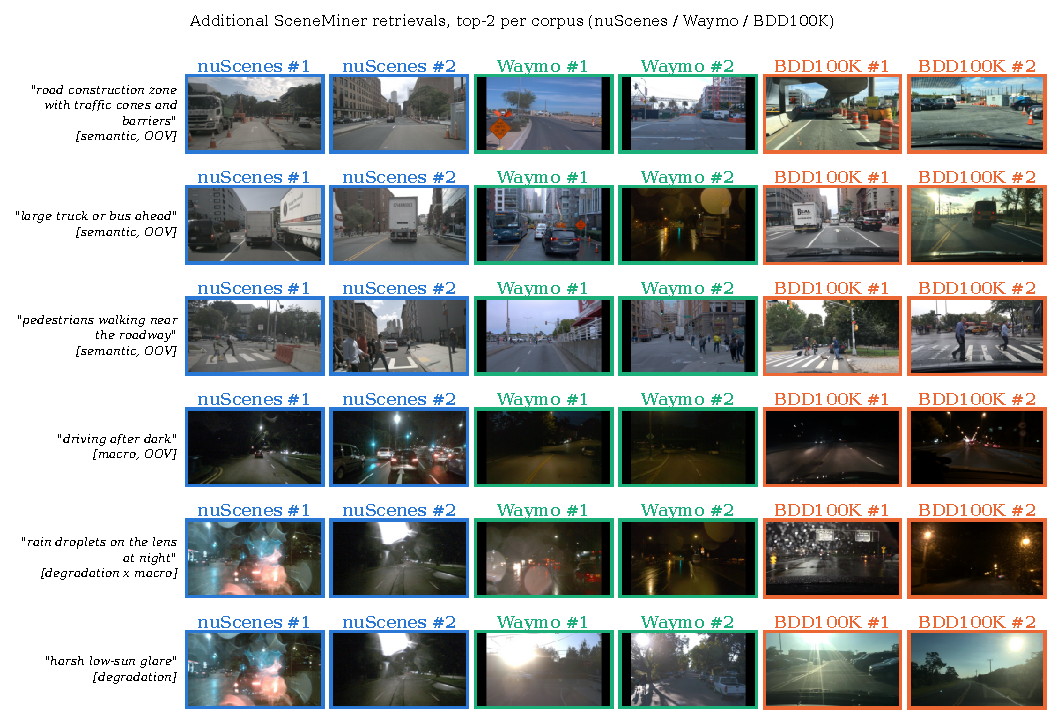
\includegraphics[width=\textwidth]{figures/supp_strips.pdf}
\caption{\textbf{Top-2 retrievals per corpus} for four degradation queries
(v2.3) and two semantic queries (v2.3A in monocular mode, because the BEV and tag
channels are contaminated for object queries on these scenes). Note the last
row: ``large truck or bus ahead'' still pulls rainy nuScenes scenes, because
that query's specificity $\gamma=0.42$ leaves part of the margin channel active.}
\label{fig:strips}
\end{figure}

\begin{figure}[!ht]\centering
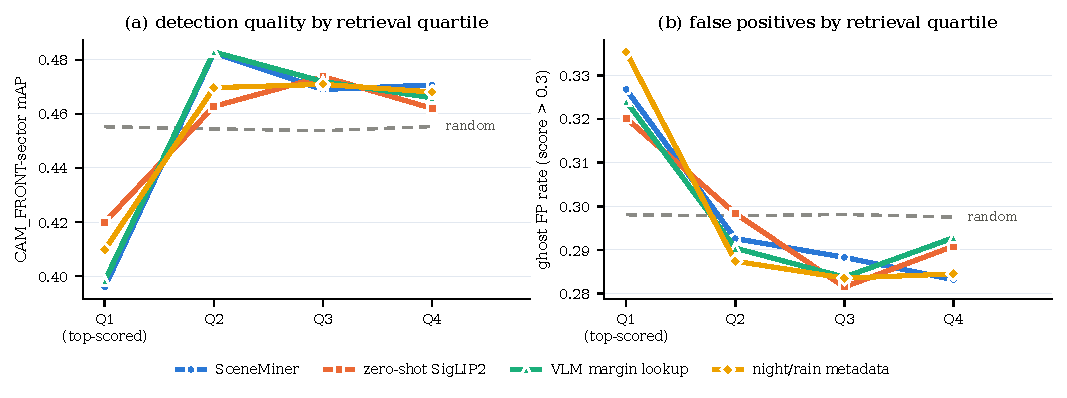
\includegraphics[width=\textwidth]{figures/fig_val150_quartiles.pdf}
\caption{\textbf{val150 retrieval quartiles}, $62$ suite degradation queries,
portable signals only. CAM\_FRONT-sector mAP (a) and ghost false-positive rate
at score $>0.3$ (b) of the scenes each ranker places in each score quartile.}
\label{fig:quart}
\end{figure}

\clearpage
% =====================================================================
\section{Training queries (not scored)}
\label{sec:train}
% =====================================================================

{\footnotesize
\begin{longtable}{r l p{8.6cm} p{5.6cm}}
\caption{The 240 training queries of the 390-query suite. They are listed for completeness and \emph{not scored}: SceneMiner's head saw their text during training.}\label{tab:train-q}\\
\toprule
\# & S & training query & predicate\\
\midrule
\endfirsthead
\toprule
\# & S & training query & predicate\\
\midrule
\endhead
\bottomrule
\endfoot
1 & S1 & heavy rain spatter obscuring the camera & droplets=T\\
2 & S1 & the lens drowned in rain streaks & droplets=T\\
3 & S1 & drizzle marking the lens & droplets=T\\
4 & S1 & persistent droplet smear on the glass & droplets=T\\
5 & S1 & strong headlight bloom from oncoming traffic & glare=T\\
6 & S1 & blinding light bloom swallowing the scene & glare=T\\
7 & S1 & harsh low-sun glare & glare=T\\
8 & S1 & scattered street-light halos & glare=T\\
9 & S1 & standing water pooling on the road & wet\_road=T\\
10 & S1 & a soaked roadway with mirror-like sheen & wet\_road=T\\
11 & S1 & rain-slicked carriageway & wet\_road=T\\
12 & S1 & puddled road surface & wet\_road=T\\
13 & S1 & a low contrast scene where vehicles are barely distinguishable & low\_contrast=T\\
14 & S1 & murky scene with indistinct vehicle outlines & low\_contrast=T\\
15 & S1 & grey scene with little tonal separation & low\_contrast=T\\
16 & S1 & objects dissolving into the background & low\_contrast=T\\
17 & S1 & heavy rain spatter obscuring the camera in daylight & droplets=T, lighting=day\\
18 & S1 & heavy rain spatter obscuring the camera in dense traffic & droplets=T, density=dense\\
19 & S1 & heavy rain spatter obscuring the camera on an empty road & droplets=T, density=sparse\\
20 & S1 & the lens drowned in rain streaks in daylight & droplets=T, lighting=day\\
21 & S1 & the lens drowned in rain streaks in dense traffic & droplets=T, density=dense\\
22 & S1 & the lens drowned in rain streaks on an empty road & droplets=T, density=sparse\\
23 & S1 & drizzle marking the lens in daylight & droplets=T, lighting=day\\
24 & S1 & drizzle marking the lens in dense traffic & droplets=T, density=dense\\
25 & S1 & drizzle marking the lens on an empty road & droplets=T, density=sparse\\
26 & S1 & persistent droplet smear on the glass in daylight & droplets=T, lighting=day\\
27 & S1 & persistent droplet smear on the glass in dense traffic & droplets=T, density=dense\\
28 & S1 & persistent droplet smear on the glass on an empty road & droplets=T, density=sparse\\
29 & S1 & strong headlight bloom from oncoming traffic in daylight & glare=T, lighting=day\\
30 & S1 & strong headlight bloom from oncoming traffic in dense traffic & glare=T, density=dense\\
31 & S1 & strong headlight bloom from oncoming traffic on an empty road & glare=T, density=sparse\\
32 & S1 & blinding light bloom swallowing the scene in daylight & glare=T, lighting=day\\
33 & S1 & blinding light bloom swallowing the scene in dense traffic & glare=T, density=dense\\
34 & S1 & blinding light bloom swallowing the scene on an empty road & glare=T, density=sparse\\
35 & S1 & harsh low-sun glare in daylight & glare=T, lighting=day\\
36 & S1 & harsh low-sun glare in dense traffic & glare=T, density=dense\\
37 & S1 & harsh low-sun glare on an empty road & glare=T, density=sparse\\
38 & S1 & scattered street-light halos in daylight & glare=T, lighting=day\\
39 & S1 & scattered street-light halos in dense traffic & glare=T, density=dense\\
40 & S1 & scattered street-light halos on an empty road & glare=T, density=sparse\\
41 & S1 & standing water pooling on the road in daylight & wet\_road=T, lighting=day\\
42 & S1 & standing water pooling on the road in dense traffic & wet\_road=T, density=dense\\
43 & S1 & standing water pooling on the road on an empty road & wet\_road=T, density=sparse\\
44 & S1 & a soaked roadway with mirror-like sheen in daylight & wet\_road=T, lighting=day\\
45 & S1 & a soaked roadway with mirror-like sheen in dense traffic & wet\_road=T, density=dense\\
46 & S1 & a soaked roadway with mirror-like sheen on an empty road & wet\_road=T, density=sparse\\
47 & S1 & rain-slicked carriageway in daylight & wet\_road=T, lighting=day\\
48 & S1 & rain-slicked carriageway in dense traffic & wet\_road=T, density=dense\\
49 & S1 & rain-slicked carriageway on an empty road & wet\_road=T, density=sparse\\
50 & S1 & puddled road surface in daylight & wet\_road=T, lighting=day\\
51 & S1 & puddled road surface in dense traffic & wet\_road=T, density=dense\\
52 & S1 & puddled road surface on an empty road & wet\_road=T, density=sparse\\
53 & S1 & a low contrast scene where vehicles are barely distinguishable in daylight & low\_contrast=T, lighting=day\\
54 & S1 & a low contrast scene where vehicles are barely distinguishable in dense traffic & low\_contrast=T, density=dense\\
55 & S1 & a low contrast scene where vehicles are barely distinguishable on an empty road & low\_contrast=T, density=sparse\\
56 & S1 & murky scene with indistinct vehicle outlines in daylight & low\_contrast=T, lighting=day\\
57 & S1 & murky scene with indistinct vehicle outlines in dense traffic & low\_contrast=T, density=dense\\
58 & S1 & murky scene with indistinct vehicle outlines on an empty road & low\_contrast=T, density=sparse\\
59 & S1 & grey scene with little tonal separation in daylight & low\_contrast=T, lighting=day\\
60 & S1 & grey scene with little tonal separation in dense traffic & low\_contrast=T, density=dense\\
61 & S1 & grey scene with little tonal separation on an empty road & low\_contrast=T, density=sparse\\
62 & S1 & objects dissolving into the background in daylight & low\_contrast=T, lighting=day\\
63 & S1 & objects dissolving into the background in dense traffic & low\_contrast=T, density=dense\\
64 & S1 & objects dissolving into the background on an empty road & low\_contrast=T, density=sparse\\
65 & S2 & night driving on an unlit road & lighting=night\\
66 & S2 & the street under lamplight & lighting=night\\
67 & S2 & driving under full daylight & lighting=day\\
68 & S2 & an afternoon street view & lighting=day\\
69 & S2 & rainfall over the roadway & weather=rain\\
70 & S2 & driving through a shower & weather=rain\\
71 & S2 & driving in settled weather & weather=dry\\
72 & S2 & a rain-free street & weather=dry\\
73 & S2 & queued vehicles filling the lane & density=dense\\
74 & S2 & packed traffic ahead & density=dense\\
75 & S2 & an open road with few cars & density=sparse\\
76 & S2 & a near-empty carriageway & density=sparse\\
77 & S2 & steady but unhurried traffic & density=moderate\\
78 & S2 & a handful of cars on the road & density=moderate\\
79 & S1 & a few water specks on the lens, seen in daylight & droplets=T, lighting=day\\
80 & S1 & a few water specks on the lens, seen in dense traffic & droplets=T, density=dense\\
81 & S1 & a few water specks on the lens, seen on an empty road & droplets=T, density=sparse\\
82 & S1 & light droplets scattered on the lens, seen in daylight & droplets=T, lighting=day\\
83 & S1 & light droplets scattered on the lens, seen in dense traffic & droplets=T, density=dense\\
84 & S1 & light droplets scattered on the lens, seen on an empty road & droplets=T, density=sparse\\
85 & S1 & water droplets smearing the camera lens, seen in daylight & droplets=T, lighting=day\\
86 & S1 & water droplets smearing the camera lens, seen in dense traffic & droplets=T, density=dense\\
87 & S1 & water droplets smearing the camera lens, seen on an empty road & droplets=T, density=sparse\\
88 & S1 & rain beading across the lens, seen in daylight & droplets=T, lighting=day\\
89 & S1 & rain beading across the lens, seen in dense traffic & droplets=T, density=dense\\
90 & S1 & rain beading across the lens, seen on an empty road & droplets=T, density=sparse\\
91 & S1 & a faint halo around a street light, seen in daylight & glare=T, lighting=day\\
92 & S1 & a faint halo around a street light, seen in dense traffic & glare=T, density=dense\\
93 & S1 & a faint halo around a street light, seen on an empty road & glare=T, density=sparse\\
94 & S1 & mild light flare at the frame edge, seen in daylight & glare=T, lighting=day\\
95 & S1 & mild light flare at the frame edge, seen in dense traffic & glare=T, density=dense\\
96 & S1 & mild light flare at the frame edge, seen on an empty road & glare=T, density=sparse\\
97 & S1 & noticeable glare washing across the image, seen in daylight & glare=T, lighting=day\\
98 & S1 & noticeable glare washing across the image, seen in dense traffic & glare=T, density=dense\\
99 & S1 & noticeable glare washing across the image, seen on an empty road & glare=T, density=sparse\\
100 & S1 & specular glare washing out the image, seen in daylight & glare=T, lighting=day\\
101 & S1 & specular glare washing out the image, seen in dense traffic & glare=T, density=dense\\
102 & S1 & specular glare washing out the image, seen on an empty road & glare=T, density=sparse\\
103 & S1 & a lightly damp road surface, seen in daylight & wet\_road=T, lighting=day\\
104 & S1 & a lightly damp road surface, seen in dense traffic & wet\_road=T, density=dense\\
105 & S1 & a lightly damp road surface, seen on an empty road & wet\_road=T, density=sparse\\
106 & S1 & patchy wet tarmac, seen in daylight & wet\_road=T, lighting=day\\
107 & S1 & patchy wet tarmac, seen in dense traffic & wet\_road=T, density=dense\\
108 & S1 & patchy wet tarmac, seen on an empty road & wet\_road=T, density=sparse\\
109 & S1 & wet reflective asphalt after rainfall, seen in daylight & wet\_road=T, lighting=day\\
110 & S1 & wet reflective asphalt after rainfall, seen in dense traffic & wet\_road=T, density=dense\\
111 & S1 & wet reflective asphalt after rainfall, seen on an empty road & wet\_road=T, density=sparse\\
112 & S1 & slick wet pavement throwing reflections, seen in daylight & wet\_road=T, lighting=day\\
113 & S1 & slick wet pavement throwing reflections, seen in dense traffic & wet\_road=T, density=dense\\
114 & S1 & slick wet pavement throwing reflections, seen on an empty road & wet\_road=T, density=sparse\\
115 & S1 & slightly flat lighting, seen in daylight & low\_contrast=T, lighting=day\\
116 & S1 & slightly flat lighting, seen in dense traffic & low\_contrast=T, density=dense\\
117 & S1 & slightly flat lighting, seen on an empty road & low\_contrast=T, density=sparse\\
118 & S1 & a dim view where shapes lose definition, seen in daylight & low\_contrast=T, lighting=day\\
119 & S1 & a dim view where shapes lose definition, seen in dense traffic & low\_contrast=T, density=dense\\
120 & S1 & a dim view where shapes lose definition, seen on an empty road & low\_contrast=T, density=sparse\\
121 & S1 & hazy washed out view with unclear boundaries, seen in daylight & low\_contrast=T, lighting=day\\
122 & S1 & hazy washed out view with unclear boundaries, seen in dense traffic & low\_contrast=T, density=dense\\
123 & S1 & hazy washed out view with unclear boundaries, seen on an empty road & low\_contrast=T, density=sparse\\
124 & S1 & poor visibility with objects blending in, seen in daylight & low\_contrast=T, lighting=day\\
125 & S1 & poor visibility with objects blending in, seen in dense traffic & low\_contrast=T, density=dense\\
126 & S1 & poor visibility with objects blending in, seen on an empty road & low\_contrast=T, density=sparse\\
127 & S2 & a scene showing driving after dark & lighting=night\\
128 & S2 & a scene showing a night-time street scene & lighting=night\\
129 & S2 & a scene showing low ambient light driving & lighting=night\\
130 & S2 & a scene showing night driving on an unlit road & lighting=night\\
131 & S2 & a scene showing the street under lamplight & lighting=night\\
132 & S2 & a scene showing bright daytime driving & lighting=day\\
133 & S2 & a scene showing a clear daylight street & lighting=day\\
134 & S2 & a scene showing a midday road scene & lighting=day\\
135 & S2 & a scene showing driving under full daylight & lighting=day\\
136 & S2 & a scene showing an afternoon street view & lighting=day\\
137 & S2 & a scene showing driving in rain & weather=rain\\
138 & S2 & a scene showing a rainy street & weather=rain\\
139 & S2 & a scene showing wet weather driving & weather=rain\\
140 & S2 & a scene showing rainfall over the roadway & weather=rain\\
141 & S2 & a scene showing driving through a shower & weather=rain\\
142 & S2 & a scene showing dry road conditions & weather=dry\\
143 & S2 & a scene showing a dry clear day & weather=dry\\
144 & S2 & a scene showing no precipitation on the road & weather=dry\\
145 & S2 & a scene showing driving in settled weather & weather=dry\\
146 & S2 & a scene showing a rain-free street & weather=dry\\
147 & S2 & a scene showing dense bumper-to-bumper traffic & density=dense\\
148 & S2 & a scene showing a congested roadway & density=dense\\
149 & S2 & a scene showing a heavy traffic jam & density=dense\\
150 & S2 & a scene showing queued vehicles filling the lane & density=dense\\
151 & S2 & a scene showing packed traffic ahead & density=dense\\
152 & S2 & a scene showing an almost empty road & density=sparse\\
153 & S2 & a scene showing sparse traffic & density=sparse\\
154 & S2 & a scene showing a deserted street & density=sparse\\
155 & S2 & a scene showing an open road with few cars & density=sparse\\
156 & S2 & a scene showing a near-empty carriageway & density=sparse\\
157 & S2 & a scene showing a moderately busy road & density=moderate\\
158 & S2 & a scene showing a few vehicles around & density=moderate\\
159 & S2 & a scene showing light traffic flow & density=moderate\\
160 & S2 & a scene showing steady but unhurried traffic & density=moderate\\
161 & S2 & a scene showing a handful of cars on the road & density=moderate\\
162 & S2 & footage of driving after dark & lighting=night\\
163 & S2 & footage of a night-time street scene & lighting=night\\
164 & S2 & footage of low ambient light driving & lighting=night\\
165 & S2 & footage of night driving on an unlit road & lighting=night\\
166 & S2 & footage of the street under lamplight & lighting=night\\
167 & S2 & footage of bright daytime driving & lighting=day\\
168 & S2 & footage of a clear daylight street & lighting=day\\
169 & S2 & footage of a midday road scene & lighting=day\\
170 & S2 & footage of driving under full daylight & lighting=day\\
171 & S2 & footage of an afternoon street view & lighting=day\\
172 & S2 & footage of driving in rain & weather=rain\\
173 & S2 & footage of a rainy street & weather=rain\\
174 & S2 & footage of wet weather driving & weather=rain\\
175 & S2 & footage of rainfall over the roadway & weather=rain\\
176 & S2 & footage of driving through a shower & weather=rain\\
177 & S2 & footage of dry road conditions & weather=dry\\
178 & S2 & footage of a dry clear day & weather=dry\\
179 & S2 & footage of no precipitation on the road & weather=dry\\
180 & S2 & footage of driving in settled weather & weather=dry\\
181 & S2 & footage of a rain-free street & weather=dry\\
182 & S2 & footage of dense bumper-to-bumper traffic & density=dense\\
183 & S2 & footage of a congested roadway & density=dense\\
184 & S2 & footage of a heavy traffic jam & density=dense\\
185 & S2 & footage of queued vehicles filling the lane & density=dense\\
186 & S2 & footage of packed traffic ahead & density=dense\\
187 & S2 & footage of an almost empty road & density=sparse\\
188 & S2 & footage of sparse traffic & density=sparse\\
189 & S2 & footage of a deserted street & density=sparse\\
190 & S2 & footage of an open road with few cars & density=sparse\\
191 & S2 & footage of a near-empty carriageway & density=sparse\\
192 & S2 & footage of a moderately busy road & density=moderate\\
193 & S2 & footage of a few vehicles around & density=moderate\\
194 & S2 & footage of light traffic flow & density=moderate\\
195 & S2 & footage of steady but unhurried traffic & density=moderate\\
196 & S2 & footage of a handful of cars on the road & density=moderate\\
197 & S1 & a recording with a few water specks on the lens & droplets=T\\
198 & S1 & a recording with light droplets scattered on the lens & droplets=T\\
199 & S1 & a recording with water droplets smearing the camera lens & droplets=T\\
200 & S1 & a recording with rain beading across the lens & droplets=T\\
201 & S1 & a recording with heavy rain spatter obscuring the camera & droplets=T\\
202 & S1 & a recording with the lens drowned in rain streaks & droplets=T\\
203 & S1 & a recording with drizzle marking the lens & droplets=T\\
204 & S1 & a recording with persistent droplet smear on the glass & droplets=T\\
205 & S1 & a recording with a faint halo around a street light & glare=T\\
206 & S1 & a recording with mild light flare at the frame edge & glare=T\\
207 & S1 & a recording with noticeable glare washing across the image & glare=T\\
208 & S1 & a recording with specular glare washing out the image & glare=T\\
209 & S1 & a recording with strong headlight bloom from oncoming traffic & glare=T\\
210 & S1 & a recording with blinding light bloom swallowing the scene & glare=T\\
211 & S1 & a recording with harsh low-sun glare & glare=T\\
212 & S1 & a recording with scattered street-light halos & glare=T\\
213 & S1 & a recording with a lightly damp road surface & wet\_road=T\\
214 & S1 & a recording with patchy wet tarmac & wet\_road=T\\
215 & S1 & a recording with wet reflective asphalt after rainfall & wet\_road=T\\
216 & S1 & a recording with slick wet pavement throwing reflections & wet\_road=T\\
217 & S1 & a recording with standing water pooling on the road & wet\_road=T\\
218 & S1 & a recording with a soaked roadway with mirror-like sheen & wet\_road=T\\
219 & S1 & a recording with rain-slicked carriageway & wet\_road=T\\
220 & S1 & a recording with puddled road surface & wet\_road=T\\
221 & S1 & a recording with slightly flat lighting & low\_contrast=T\\
222 & S1 & a recording with a dim view where shapes lose definition & low\_contrast=T\\
223 & S1 & a recording with hazy washed out view with unclear boundaries & low\_contrast=T\\
224 & S1 & a recording with poor visibility with objects blending in & low\_contrast=T\\
225 & S1 & a recording with a low contrast scene where vehicles are barely distinguishable & low\_contrast=T\\
226 & S1 & a recording with murky scene with indistinct vehicle outlines & low\_contrast=T\\
227 & S1 & a recording with grey scene with little tonal separation & low\_contrast=T\\
228 & S1 & a recording with objects dissolving into the background & low\_contrast=T\\
229 & S1 & dashcam footage showing a few water specks on the lens & droplets=T\\
230 & S1 & dashcam footage showing light droplets scattered on the lens & droplets=T\\
231 & S1 & dashcam footage showing water droplets smearing the camera lens & droplets=T\\
232 & S1 & dashcam footage showing rain beading across the lens & droplets=T\\
233 & S1 & dashcam footage showing heavy rain spatter obscuring the camera & droplets=T\\
234 & S1 & dashcam footage showing the lens drowned in rain streaks & droplets=T\\
235 & S1 & dashcam footage showing drizzle marking the lens & droplets=T\\
236 & S1 & dashcam footage showing persistent droplet smear on the glass & droplets=T\\
237 & S1 & dashcam footage showing a faint halo around a street light & glare=T\\
238 & S1 & dashcam footage showing mild light flare at the frame edge & glare=T\\
239 & S1 & dashcam footage showing noticeable glare washing across the image & glare=T\\
240 & S1 & dashcam footage showing specular glare washing out the image & glare=T\\
\end{longtable}

}

% =====================================================================
\section{Reproduction}
% =====================================================================

{\small
\begin{verbatim}
scripts/launch_seeds.sh scripts/train_sceneminer_v23.py work_dirs/sceneminer_v23 v23
python scripts/eval_v23.py                   # human GT, BDD100K, suite, ablations
python scripts/extract_human_semantic_gt.py
python scripts/build_semantic_queries.py
python scripts/eval_semantic_edge_cases.py   # Stratum 5, corpus + clean val150
python scripts/val150_camfront_errors.py     # front-sector degradation study
python scripts/val150_ped_vru_metrics.py
python scripts/val150_retrieval_to_3d.py     # retrieval -> breakage loop
python scripts/make_figures.py && python scripts/make_supp_tables.py
\end{verbatim}
}

\end{document}
